\section{实验原理}
尽管仪器可以测出各个测点相对总基点间的重力差值,但引起各测点相对总基点间的重力差值的原理有很多,除了地下因素以外,还有各测点相对总基点的纬度变化、高程变化及测点周围地形起伏等因素。
\begin{equation}
\label{gravity}
	\varDelta g_A=\varDelta g_{A-G}-\varDelta g_{\varphi}-\varDelta g_h-\varDelta g_m-\varDelta g_t
\end{equation}

式中:$\varDelta g_A$为地质体剩余质量在$A$点产生的重力异常;$g_{\varphi}$为测点相对于基点$G$的纬度影响;$\varDelta g_h$为测点相对于基点$G$的高度影响;$\varDelta g_m$为测点与基点$G$之间物质层(中间层)对$A$点的影响;$\varDelta g_t$为$A$点周围地形的影响。

\subsection{纬度校正}
由于正常重力值是纬度$\varphi$的函数,当测点与总基点纬度不同时,所产生的纬度影响也不同,消除纬度影响称为纬度改正。

当纬度变化不大时,正常重力值随纬度的变化,可直接用正常重力公式$g_{\varphi}=9780490\\ \left( 1+\text{0.0052884}\sin ^2\varphi -\text{0.0000059}\sin ^2\phi \right) \left( g.u. \right) $的全微分来代替。忽略上式中的第三项,对$\varphi$求微分后课得到
\begin{equation}
\label{latitude 1}
\varDelta g_{\varphi}=\frac{\partial \varDelta g_{\phi}}{\partial \varphi}\varDelta \phi =\text{51855.1506}\sin 2\phi \cdot \varDelta \phi 
\end{equation}

在$\varDelta \phi$较小时,$\varDelta \phi$可以用测点到总基点间纬向(南北向)距离$D$来表示,$D$、$\varDelta \phi$和地球半径$R$的关系为$\varDelta \phi =D/R$,若取$R=6370.8km$,并将它带入公式\ref{latitude 1},便有
\begin{equation}
	\varDelta g_{\varphi}=-\text{8.14}\sin ^2\phi \cdot D\,\,\left( g.u. \right) 
\end{equation}


公式前面另外加上的负号表示其作为校正公式可直接带入公式\ref{gravity}中进行计算。式中$\varphi$为测区的平均纬度,$D$表示测点与总基点的纬向距离。对北半球而言,当测点在总基点以北时,纬度影响为正,$D$取正值;测点在总基点以南时,纬度影响值为负,$D$取负值,其单位为km。
\subsection{地形改正}
\subsubsection{地形影响因素的理论计算}
地形对测点的重力影响永远是为负值,也就是说它使重力值减小,所以,地形改正值永远为正值。
\begin{figure}
	\centering
	\label{dixingyingxiangshiyitu}
	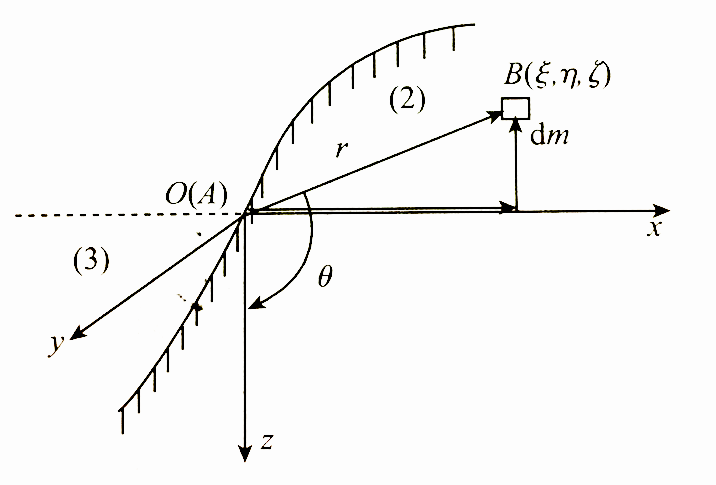
\includegraphics[scale = 0.7]{figures/dixingjiaozhengyuanli1.png}
	\caption{地形影响示意图}
\end{figure}

取直角坐标系,如图\ref{dixingyingxiangshiyitu}所示,并将测点$A$所在的位置定位原点,$z$轴垂直向下,$x$、$y$轴在$A$点所在的水平面内。$dm$为质量元,其所在的$B$点坐标为$\left( \xi ,\eta ,\zeta \right) $;$A$点到$B$点矢径用\textbf{r}表示,$r$与$z$轴夹角为$\theta$。$dm$在$A$点产生的重力影响,即引力的垂直分量为
\begin{equation}
	dg=G\frac{dm}{r^2}\cos \vartheta 
\end{equation}

式中:$r\,\,=\,\,\left( \xi ^2+\eta ^2+\zeta ^2 \right)$;$dm\,\,=\,\,\rho \cdot d\xi d\eta d\zeta $;$\cos \vartheta \,\,=\,\,\frac{\zeta}{r}$,其中$\zeta$为负值。

由图\ref{dixingyingxiangshiyitu}可知,若计算区域$\left( 2 \right)$全部质量的影响可用积分计算,
\begin{equation}
	\varDelta g\,\,=\,\,G\iiiint_V{\frac{\zeta \rho}{\left( \xi ^2+\eta ^2+\zeta ^2 \right) ^{\text{3/}2}}d\xi d\eta d\zeta}
\end{equation}
\subsubsection{地形影响因素的近似计算}
目前地形改正值的计算有两种分割方法,一是用扇形柱体分割地形,二是用方柱体分割地形。前者适用于量板计算,后者用于计算机编程计算。

地改范围一般为:$\text{0~}20m$为近区,$\text{20~}400m$为中区,$400m$到最大地改范围为远区。

\begin{enumerate}
	\item 扇形域地形改正值计算法:首先在地形图上以测点$A$为圆心,以不同半径$R$作圆环,然后通过$A$点安等角度作辐射线分割各圆环,图\ref{扇形域划分图}中阴影面积即为其中一个扇形柱体的截面积。图\ref{扇形柱体地形校正计算图}为一个扇形柱体相对$A$点的位置关系。柱体的高度有地形图中读取。实际工作中,扇形柱体的高度$h$为地形平均高程与测点高程之差。若计算任一扇形柱体在$A$点的改正值,可在柱坐标系中完成。由于$d\xi d\eta d\zeta = Rd\alpha \cdot dR\cdot d\xi $,$\xi ^2+\eta ^2=R^2$,令$\alpha _{i+1}-\alpha _i=2\pi /n$,则
	\begin{equation}
		\varDelta g_{t}^{‘}=\frac{2\pi G\rho}{n}\left( \sqrt{R_{i}^{2}+h^2}-R_i-\sqrt{R_{i+1}^{2}+h^2}+R_{i+1} \right) 
	\end{equation}
	
	最后把$A$点周围所有扇形柱体都计算出来,相加之后就得到总改正值,即
	\begin{equation}
		\varDelta g_{\text{地改}}=\sum_{i=1}^n{\varDelta g_{t_i}^{’}}
	\end{equation}
	
	\begin{figure}[htbp]
		\centering
		%\subfigure[]
		{
			\begin{minipage}{7cm}
				\centering
				\label{扇形域划分图}
				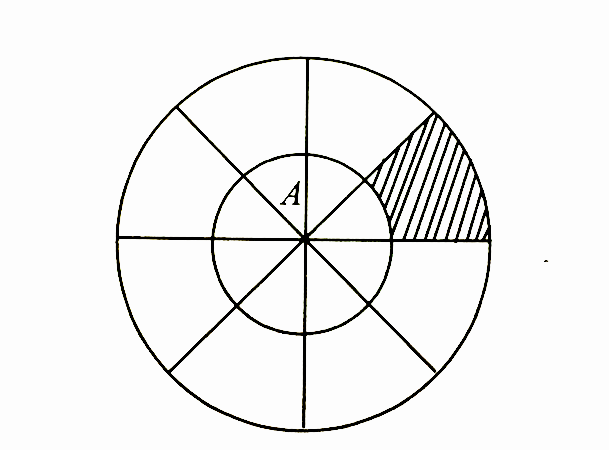
\includegraphics[scale = 0.7]{figures/dixingjiaozhengyuanli.png}
				\caption{扇形域划分图}
			\end{minipage}
		}
		%\subfigure[]
		{
			\begin{minipage}{7cm}
				\centering
				\label{扇形柱体地形校正计算图}
				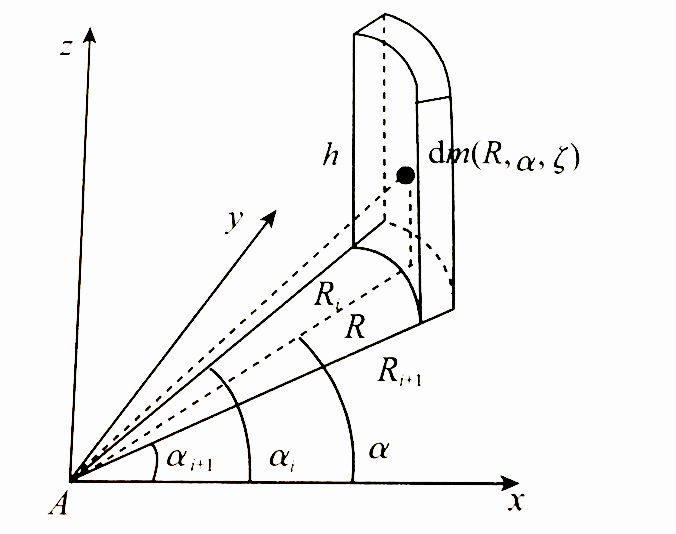
\includegraphics[scale = 0.7]{figures/zhongyuanqu.png}
				\caption{扇形柱体地形校正计算图}
			\end{minipage}
		}
	\end{figure}
	
	\item 近区扇形锥体的地形改正值计算法:图\ref{锥体地形校正图}表示一个扇形锥体。$A$为测点,$h$为扇形锥体的高度,$R$为测点$A$到$B$点的水平距离,$i$为锥面倾角。由于$h=R\cdot \tan i$,所以,锥体的地形改正值为
	
	\begin{equation}
		\varDelta g_{t}^{‘}  =G\rho \int_0^R{\int_{\alpha _i}^{\alpha _{i+1}}{\int_0^{R\tan i}{\frac{R\zeta}{\left( R^2+\zeta ^2 \right) ^{\text{3/}2}}dRd\zeta d\alpha}} =G\left( \alpha _{i+1}-\alpha _i \right) \left[ R\left( 1-\cos i \right) \right]}
	\end{equation}
	
	\begin{figure}
		\centering
		\label{锥体地形校正图}
		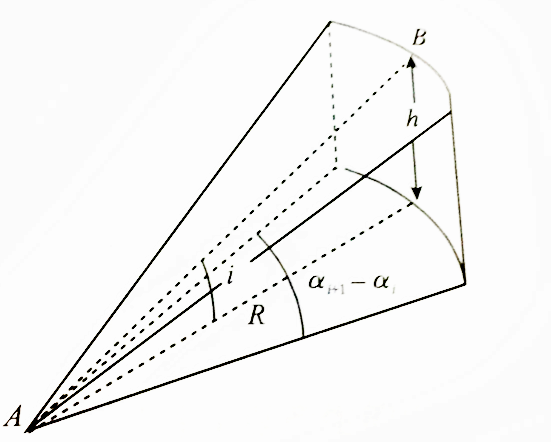
\includegraphics[scale = 0.7]{figures/jinqu.png}
		\caption{锥体地形校正计算图}
	\end{figure}
	\item 
	\begin{figure}
		\centering
		\label{fangxing}
		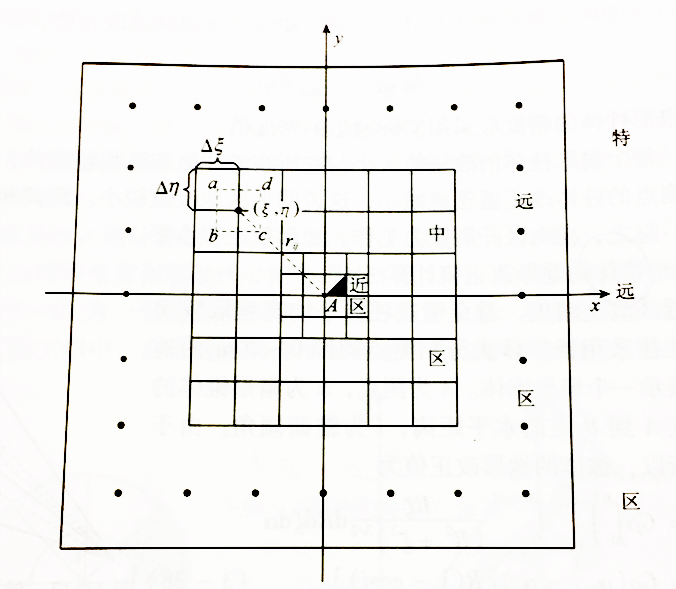
\includegraphics[scale = 0.7]{figures/fangxing.png}
		\caption{方形域地形校正分区计算示意图}
	\end{figure}

	图\ref{fangxing}是用方形域分割测点周围地形的示意图。其中网格节点为重力测点。若$A$测点的坐标为$\left( \text{0,0,}h_0 \right)$,方形域柱体所代表的面积元与网格面积相等,其中心点水平坐标为$\left( \xi _i,\eta _i \right) $,方形柱平均高程与$A$点高程之差为$h_{i,j}$,则全部地形改正值可表示为
	\begin{equation}
		\varDelta g_t=\sum_{i\,\,=1}^n{\sum_{j=1}^n{\frac{K_{ij}}{r_{ij}}\left\{ 1-\left[ 1+\left( \frac{h_{ij}}{r_{ij}} \right) ^2 \right] ^{-\text{1/}2} \right\}}}
	\end{equation}
	
	式中,$K_{ij}$为各方柱体所应用的系数,$r_{ij}$表示柱体到地改点的距离。
\end{enumerate}
\subsubsection{地改范围}
设$\varepsilon $为重力异常精度,为了满足$\varDelta g_T\leqslant \varepsilon $,则需
\begin{equation}
R_i\geqslant \frac{\pi G\rho h^2}{\varepsilon}
\end{equation}

式中,$h$为$R_i$以外地形平均高差;$R_i$为地改最大半径。
\subsection{中间层改正}
经过地形改正后可认为测点周围平坦了,但测点$A$所在的平面和基点相比仍高$h$,亦即测点仍处于一个半径为$R$(地改范围),厚度为$h$,密度为$rho$的圆盘上。这个圆盘(中间层)同样要产生影响,消除这个影响,叫做中间层改正。
\begin{figure}
	\centering
	\label{zjc}
	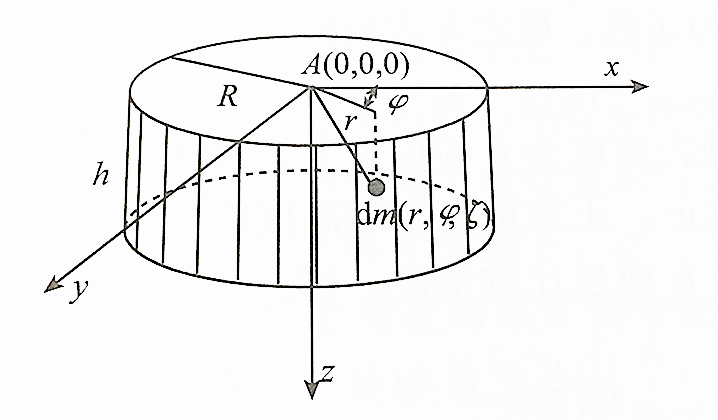
\includegraphics[scale = 0.7]{figures/mlayer.png}
	\caption{计算圆盘在A点产生的引力垂直分量图}
\end{figure}

由公式知中间层对$A$点产生的引力影响值$\varDelta g_m$:
\begin{equation}
	\varDelta g=G\int{\int_V{\frac{dm}{r^2}\cos \theta}=G\int{\int_V{\frac{\zeta \rho}{\left( \xi ^2+\eta ^2+\zeta ^2 \right) ^{\text{3/}2}}d\xi d\eta d\zeta}}}
\end{equation}
将上述方程中个物理量选择特定单位后,该公式可进一步改写为:
\begin{equation}
	\varDelta g_m=-\left[ 0.419-\frac{0.2095}{\left\{ R \right\} _m}\left\{ h \right\} _m \right] \left\{ \rho \right\} _{g\cdot cm^{-3}}\left\{ h \right\} _m\left( g.u. \right) 
\end{equation}

上式中等号右端下脚标表示该量选定的单位,$\{\}$中表示该量的数值。式中$h$为测点与总基点之间的高差,当测点高于基点时$h$为正值,反之为负值。
\subsection{高度改正}
经过中间层改正后,测点相对基点而言仍处于高度为$h$的位置上,对于这个高度影响要予以消除。正常重力场随高度的变化值可近似的方法求得,即$g=C\frac{1}{R^2}$,式中,$C$为比例常数,将上式对$R$求导得到正常重力场随$R$的变化率 $\frac{\partial g}{\partial R}=\frac{-2C}{R^3}$,消去常数$C$得$\frac{\partial g}{\partial R}=\frac{-2C}{R}$,取$R=6370\times 10^3m
$和$g=9.8\times 10^6\,\,g.u.
$代入后得$\frac{\partial g}{\partial R}=-\text{3.086 }g.u.
$,也就是说测点每升高1m时,正常重力值将减小$3,086(g.u.)$。

高度改正值$\varDelta g_{\text{高}}$:应为
\begin{equation}
	\varDelta g_{\text{高}}=3.086\left\{ h \right\} _m\,\,\left( g.u. \right) 
\end{equation}

可利用理想大地水准面上的正常重力表达式对$R$求导而得到更精确的表达式,为
\begin{equation}
	\varDelta g_{\text{高}}=3.086\left( 1+\text{0.007}\cos 2\phi \right) \left\{ h \right\} _m-7.2\times 10^{-7}\left\{ h \right\} _{m}^{2}\,\,\left( g.u. \right) 
\end{equation}